% !TEX program = lualatex
% Compile from 2026/week11; notebooks provide the numerical figures.
\documentclass[12pt,aspectratio=43]{beamer}
% Shared Beamer design. Load after \documentclass using \input.
% Engine: LuaLaTeX. Fonts: UD Digi Kyokasho N (regular/bold), Arial.
\usepackage{luatexja-fontspec}
\setmainjfont[BoldFont={UD Digi Kyokasho N Bold}]{UD Digi Kyokasho N}
\setsansjfont[BoldFont={UD Digi Kyokasho N Bold}]{UD Digi Kyokasho N}
\setmonojfont[BoldFont={UD Digi Kyokasho N Bold}]{UD Digi Kyokasho N}
% Liberation Sans keeps the layout usable on systems without Arial.
\IfFontExistsTF{Arial}{
  \setmainfont{Arial}
  \setsansfont{Arial}
  \setmonofont{Arial}
}{
  \setmainfont{Liberation Sans}
  \setsansfont{Liberation Sans}
  \setmonofont{Liberation Sans}
}
\renewcommand{\kanjifamilydefault}{\gtdefault}

% Typeset mathematics with a dedicated TeX math font, independent of Arial.
\usefonttheme{professionalfonts}
\usepackage[mathrm=sym]{unicode-math}
\setmathfont{Latin Modern Math}
\setoperatorfont{\symup}

\definecolor{courseblue}{HTML}{4472C4}
\definecolor{ruleblue}{HTML}{8FAADC}
\setbeamercolor{normal text}{fg=black,bg=white}
\setbeamercolor{structure}{fg=courseblue}
\setbeamercolor{frametitle}{fg=black,bg=white}
\setbeamercolor{title banner}{fg=white,bg=courseblue}
\setbeamerfont{frametitle}{size=\fontsize{18}{22}\selectfont,series=\mdseries}
\setbeamerfont{quote}{shape=\upshape}
\setbeamersize{text margin left=9mm,text margin right=9mm}
\setbeamertemplate{navigation symbols}{}
\setbeamercolor{page number}{fg=gray,bg=white}
\setbeamertemplate{footline}{%
  \begin{beamercolorbox}[wd=\paperwidth,ht=2.5mm,dp=1.5mm]{page number}
    \hfill{\fontsize{8}{9}\selectfont
      \ifnum\value{framenumber}>0
        \insertframenumber\,/\,\inserttotalframenumber
      \fi}\hspace*{3mm}
  \end{beamercolorbox}}
\setbeamertemplate{headline}{%
  \hfill\textcolor{gray}{\fontsize{6}{7}\selectfont
    \hypersetup{linkcolor=gray}% Keep Beamer's title links in the header color.
    \ifnum\value{framenumber}=0 \insertshortdate\enspace\fi
    \insertshorttitle\space\insertshortsubtitle}\hspace{2mm}\vspace{1.5mm}}
\setbeamertemplate{frametitle}{%
  \vspace{2mm}\centering\insertframetitle\par
  \vspace{-1mm}{\color{ruleblue}\rule{.44\paperwidth}{.5pt}}\par
  \vspace{2mm}}
\setbeamercolor{itemize item}{fg=courseblue}
\setbeamercolor{itemize subitem}{fg=black}
\setbeamercolor{itemize subsubitem}{fg=black}
\setbeamertemplate{itemize item}{\textbullet}
\setbeamertemplate{itemize subitem}{\textnormal{-}}
\setbeamertemplate{itemize subsubitem}{\textnormal{-}}
\setlength{\parskip}{.45em}
\hypersetup{colorlinks=true,urlcolor=courseblue}

% Use \titlepage inside a [t,noframenumbering] frame. The background extends
% 1 mm past both page edges to avoid hairline gaps in PDF viewers.
\setbeamertemplate{title page}{%
  \vspace{2mm}
  \begin{beamercolorbox}[wd=\paperwidth,ht=43mm,dp=13mm,colsep*=1mm,center]{title banner}
    {\fontsize{32}{40}\selectfont\inserttitle\par}
    \vspace{2mm}
    {\fontsize{20}{24}\selectfont\insertsubtitle\par}
  \end{beamercolorbox}
  \vspace{10mm}
  \hfill\insertauthor
}

\graphicspath{{figures/}}
\usepackage{listings}
\usepackage{upquote}
\IfFontExistsTF{Consolas}{\newfontfamily\codefont{Consolas}}{\newfontfamily\codefont{Liberation Mono}}
\definecolor{codevalue}{HTML}{7A3E9D}
\definecolor{codebuiltin}{HTML}{006DB0}
\definecolor{codestring}{HTML}{267348}
\newcommand{\code}[1]{{\codefont #1}}
\lstdefinestyle{python}{
  language=Python,
  basicstyle=\codefont\fontsize{12}{14}\selectfont,
  keywordstyle=\color{codebuiltin},
  keywordstyle=[2]\color{codebuiltin},
  morekeywords=[2]{print,range},
  stringstyle=\color{codestring},
  showstringspaces=false,
  columns=fullflexible,
  keepspaces=true,
  upquote=true,
  tabsize=4,
  breaklines=false,
  backgroundcolor=\color{black!4},
  frame=single,framerule=0pt,framesep=1.7mm,
  xleftmargin=1.7mm,xrightmargin=1.7mm,
  aboveskip=1mm,belowskip=0.5mm,
  literate=*{0}{{{\color{codevalue}0}}}1
    {1}{{{\color{codevalue}1}}}1 {2}{{{\color{codevalue}2}}}1
    {3}{{{\color{codevalue}3}}}1 {4}{{{\color{codevalue}4}}}1
    {5}{{{\color{codevalue}5}}}1 {6}{{{\color{codevalue}6}}}1
    {7}{{{\color{codevalue}7}}}1 {8}{{{\color{codevalue}8}}}1
    {9}{{{\color{codevalue}9}}}1
}
\lstset{style=python}
\setbeamercolor{lesson note}{fg=black,bg=courseblue!9}
\newenvironment{lessonbox}
  {\begin{beamercolorbox}[wd=\linewidth,sep=1.5mm]{lesson note}}
  {\end{beamercolorbox}\par}

\title{計算物理学B}
\subtitle{第十一回：常微分方程式2}
\author{野垣 康介、藤本 悠輝}
\date{2027/1/12}
\hypersetup{pdftitle={計算物理学B 第十一回：常微分方程式2},pdfauthor={野垣 康介、藤本 悠輝}}

\begin{document}

\begin{frame}[t,noframenumbering]
  \titlepage
\end{frame}

\begin{frame}[t]{講義予定}
  \begingroup
  \setlength{\tabcolsep}{1.6mm}
  \renewcommand{\arraystretch}{1.25}
  \begin{tabular}{@{}l@{\hspace{2mm}}l@{\hspace{4mm}}l@{\hspace{2mm}}l@{}}
    10/6 & 四則演算 & 12/8 & モンテカルロ1 \\
    10/27 & 制御文（for, if） & 12/15 & モンテカルロ2 \\
    11/6（金） & 関数 & 12/22 & 微分方程式1 \\
    11/10 & 配列（NumPy） & \textcolor{courseblue}{\textbf{1/12}} &
      \textcolor{courseblue}{\textbf{微分方程式2}} \\
    11/17 & 可視化（matplotlib） & 1/19 & 偏微分方程式1 \\
    11/24 & 数値微分 & 1/26 & 偏微分方程式2 \\
    12/1 & 数値積分 & 2/2 & 根の探索 \\
    \multicolumn{2}{c}{\small 〜中間レポート〜} &
    \multicolumn{2}{c}{\small 〜期末レポート〜}
  \end{tabular}\par
  \endgroup
  \vspace{2mm}
  {\small 10/20は出張で休講。11/6（金）は火曜授業の振替。\par}
\end{frame}

\begin{frame}[t]{今日の内容}
  \begin{itemize}
    \setlength{\itemsep}{2.5mm}
    \item SciPyのODEソルバーとLorenz方程式
    \item 二重振り子の連立運動方程式
    \item 分子動力学、leapfrog法、速度Verlet法
    \item Lennard--Jones相互作用、周期境界、統計量
  \end{itemize}
\end{frame}

\begin{frame}[t]{Notebookを開く}
  \begin{itemize}
    \setlength{\itemsep}{2mm}
    \item Google Colab：\small\url{https://colab.research.google.com/?hl=ja}
    \item 今週の入口：\small\href{https://github.com/nogaki/Computational_Physics_B/tree/main/2026/week11/week11.ipynb}{2026/week11/week11.ipynb}
    \item 個別教材：\code{Lorenz.ipynb}、\code{DoublePendulum.ipynb}、\code{MolecularDynamics.ipynb}
  \end{itemize}
  \vspace{2mm}
  \begin{lessonbox}
    \textbf{Colabで開いたら「ドライブにコピーを保存」}\par
    \small 各Notebookは独立しています。計算の重いMDは粒子数とステップ数を確認してください。
  \end{lessonbox}
\end{frame}

\begin{frame}[t,fragile]{SciPyのODEソルバー}
  初期値問題
  \[
    \frac{d\mathbf{y}}{dt}=\mathbf{f}(t,\mathbf{y}),
    \qquad \mathbf{y}(t_0)=\mathbf{y}_0
  \]
  に対し、\code{solve\_ivp}を使う。
  \begin{itemize}
    \setlength{\itemsep}{1mm}
    \item 右辺は \code{fun(t, y)}。時間が第1引数
    \item 出力時刻は \code{t\_eval}。成功状態と誤差許容値も確認
  \end{itemize}
  \begin{lstlisting}
sol = solve_ivp(fun, (t0, tf), y0,
                t_eval=times)
if not sol.success:
    raise RuntimeError(sol.message)
  \end{lstlisting}
\end{frame}

\begin{frame}[t]{Lorenz方程式}
  \[
    \begin{aligned}
      \dot{x}&=\sigma(y-x),\\
      \dot{y}&=x(\rho-z)-y,\\
      \dot{z}&=xy-\beta z.
    \end{aligned}
  \]
  標準例は $\sigma=10,\ \beta=8/3,\ \rho=28$。
  \begin{itemize}
    \item 標準パラメータではカオス的な軌道を示す
    \item 初期値を少し変えると、有限時間後の軌道が異なる
  \end{itemize}
\end{frame}

\begin{frame}[t]{Lorenzアトラクター}
  \centering
  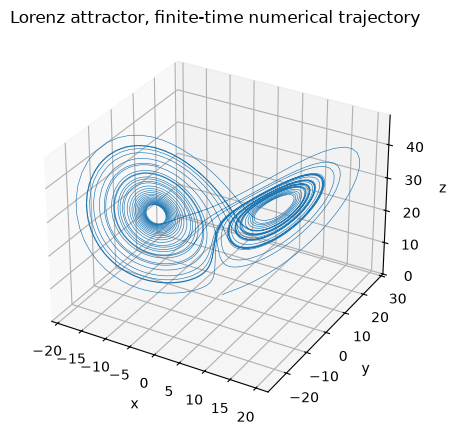
\includegraphics[width=0.60\linewidth]{lorenz_attractor.png}
\end{frame}

\begin{frame}[t]{カオスと有限時間の精度}
  \centering
  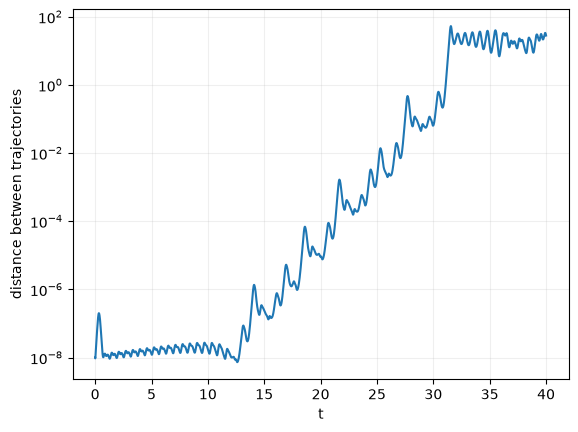
\includegraphics[width=0.67\linewidth]{lorenz_sensitivity.png}

  {\small 初期値$x_0$を$10^{-8}$だけずらした2解の距離。\par}
\end{frame}

\begin{frame}[t]{二重振り子の座標}
  \begin{columns}[T,onlytextwidth]
    \column{0.60\textwidth}
    角度は鉛直下向きから測る。支点を原点として
    \[
      \begin{aligned}
        (x_1,y_1)&=(l_1\sin\theta_1,-l_1\cos\theta_1),\\
        (x_2,y_2)&=(l_1\sin\theta_1+l_2\sin\theta_2,\\
        &\quad -l_1\cos\theta_1-l_2\cos\theta_2).
      \end{aligned}
    \]
    \column{0.37\textwidth}
    \centering
    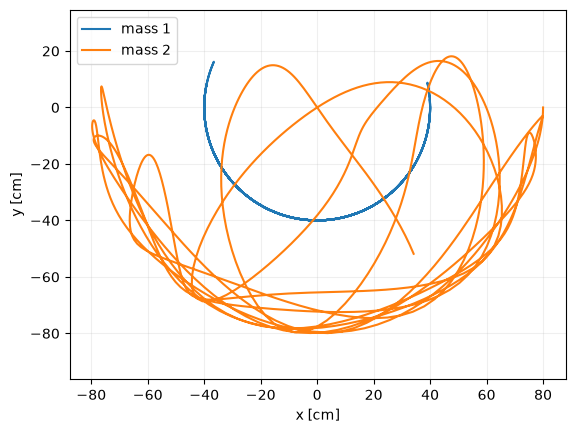
\includegraphics[width=0.9\linewidth]{double_pendulum_trace.png}
  \end{columns}
  \small 図は初期角$\theta_1=\theta_2=\pi/2$、$l_1=l_2=0.4\,\mathrm{m}$の計算結果。
\end{frame}

\begin{frame}[t]{二重振り子の運動方程式}
  $\delta=\theta_1-\theta_2$ とおくと、
  \[
    \begin{aligned}
      (m_1+m_2)l_1\ddot\theta_1
       +m_2l_2\cos\delta\,\ddot\theta_2
       &=-m_2l_2\omega_2^2\sin\delta\\
      &\quad -(m_1+m_2)g\sin\theta_1,\\
      m_2l_1\cos\delta\,\ddot\theta_1
       +m_2l_2\ddot\theta_2
       &=m_2l_1\omega_1^2\sin\delta\\
      &\quad -m_2g\sin\theta_2.
    \end{aligned}
  \]
  \small $\omega_i=\dot\theta_i$。角加速度は2元の質量行列を解いて求める。
\end{frame}

\begin{frame}[t,fragile]{4変数の1階系にする}
  \[
    \frac{d}{dt}
    \begin{pmatrix}\theta_1\\\theta_2\\\omega_1\\\omega_2\end{pmatrix}
    =
    \begin{pmatrix}\omega_1\\\omega_2\\\ddot\theta_1\\\ddot\theta_2\end{pmatrix}.
  \]
  \begin{lstlisting}
M = [[(m1+m2)*l1, m2*l2*cos(delta)],
     [m2*l1*cos(delta), m2*l2]]
alpha = np.linalg.solve(M, rhs)
  \end{lstlisting}
  \begin{itemize}
    \setlength{\itemsep}{1mm}
    \item 質量行列を直接解き、角加速度を得る
    \item solve\_ivpの右辺として時間発展させる
  \end{itemize}
\end{frame}

\begin{frame}[t]{二重振り子：数値積分の確認}
  \begin{itemize}
    \setlength{\itemsep}{1.5mm}
    \item $g=9.81\,\mathrm{m/s^2}$、$l_1=l_2=0.4\,\mathrm{m}$、$m_1=m_2=1\,\mathrm{kg}$
    \item solve\_ivpで$0\le t\le10\,\mathrm{s}$を積分
    \item 最大絶対エネルギー変動はこの実行で$1.09\times10^{-7}\,\mathrm{J}$
  \end{itemize}
  \begin{lessonbox}
    数値解でエネルギー誤差を確認する。厳密な保存を仮定せず、許容誤差や刻みを変えて結果を確かめる。
  \end{lessonbox}
\end{frame}

\begin{frame}[t]{分子動力学法}
  $N$粒子系の運動方程式を積分して、粒子の軌道と熱力学量を求める。
  \[
    m_i\ddot{\mathbf r}_i
      =\sum_{j\ne i}\mathbf F_{ij},
    \qquad
    \mathbf F_{ij}=-\nabla_i V(r_{ij})
  \]
  \begin{itemize}
    \setlength{\itemsep}{1.5mm}
    \item 周期境界を用いて有限箱からバルク系を近似
    \item 力から状態を更新し、エネルギー・温度・圧力を測る
    \item 短距離分子間相互作用の例にLennard--Jones模型を使う
  \end{itemize}
\end{frame}

\begin{frame}[t]{Lennard--Jonesポテンシャル}
  \begin{columns}[T,onlytextwidth]
    \column{0.49\textwidth}
    \[
      V_{\rm LJ}(r)=4\epsilon
      \left[\left(\frac{\sigma}{r}\right)^{12}
      -\left(\frac{\sigma}{r}\right)^6\right]
    \]
    \begin{itemize}
      \setlength{\itemsep}{1mm}
      \item 短距離で斥力、中距離で引力
      \item 最小値は$r_m=2^{1/6}\sigma$、$V=-\epsilon$
    \end{itemize}
    \column{0.49\textwidth}
    \centering
    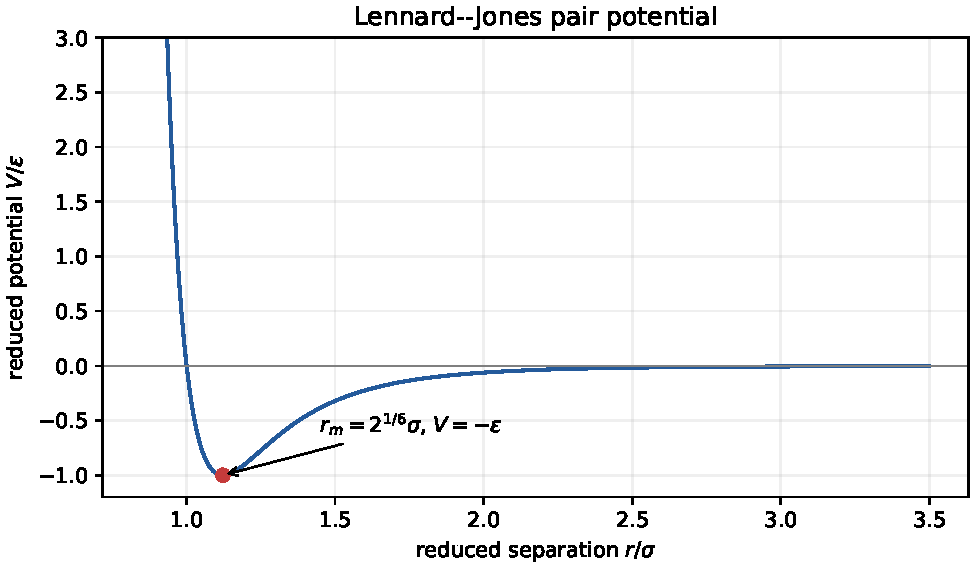
\includegraphics[width=\linewidth]{lj_potential.pdf}
  \end{columns}
\end{frame}

\begin{frame}[t]{LJ系の相図}
  \begin{columns}[T,onlytextwidth]
    \column{0.50\textwidth}
    \begin{itemize}
      \setlength{\itemsep}{2mm}
      \item 気体・液体・固体と超臨界領域
      \item 相境界や臨界点を含む多様な相転移
      \item 相図の精密計算には平衡化と統計処理が必要
    \end{itemize}
    \column{0.47\textwidth}
    \centering
    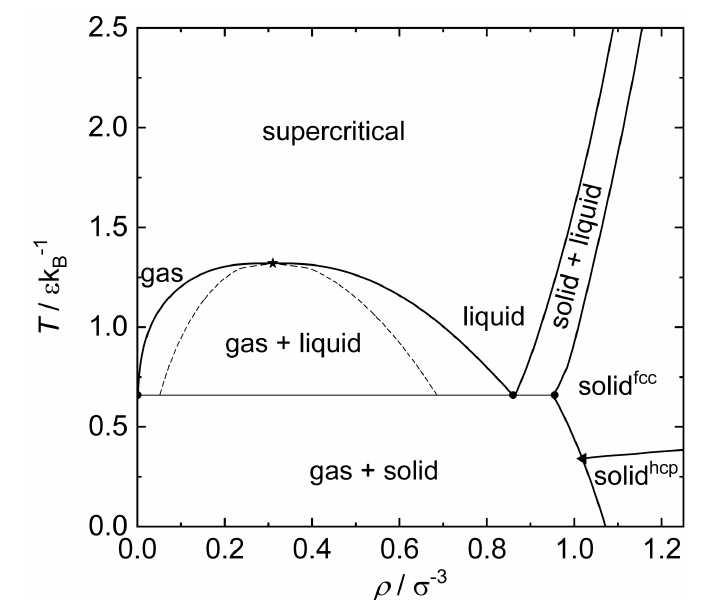
\includegraphics[width=\linewidth]{phase_diagram.png}
  \end{columns}
  \vspace{1mm}
  {\fontsize{7}{8}\selectfont 相図：S. Stephan et al., J. Chem. Inf. Model. 59, 4248 (2019)。本Notebookの短いMD計算とは別の文献図。\par}
\end{frame}

\begin{frame}[t]{換算単位}
  LJ模型では$\sigma$、$\epsilon$、$m$を単位に取れる。
  \[
    \tilde r=\frac{r}{\sigma},\qquad
    \tilde T=\frac{k_{\rm B}T}{\epsilon},\qquad
    \tilde\rho=\rho\sigma^3
  \]
  \begin{itemize}
    \setlength{\itemsep}{1.5mm}
    \item Notebookでは$\sigma=\epsilon=m=k_{\rm B}=1$
    \item 時間は$\tau=\sigma\sqrt{m/\epsilon}$を単位とする
    \item 数値は無次元化された値として読む
  \end{itemize}
\end{frame}

\begin{frame}[t]{周期境界と最小像}
  \begin{itemize}
    \setlength{\itemsep}{2mm}
    \item 粒子が箱の端を越えたら反対側へ戻す
    \item 対ごとに周期像のうち最短の差ベクトルを使う
    \item 最小像と整合するように相互作用を$r_c=L/2$で打ち切る
  \end{itemize}
  \[
    \mathbf r_{ij}^{\rm min}
       =\mathbf r_i-\mathbf r_j
        -L\,\mathrm{round}\!\left(\frac{\mathbf r_i-\mathbf r_j}{L}\right)
  \]
  \begin{lessonbox}
    Notebookではforce-shiftしたLJ相互作用を使い、$V(r_c)=0$かつ力も$r_c$で0にする。
    これは全ての周期像を足し上げる長距離LJ計算ではない。
  \end{lessonbox}
\end{frame}

\begin{frame}[t]{leapfrog法：位置と速度を半ステップずらす}
  \[
    \begin{aligned}
      \mathbf v_{n+1/2}&=\mathbf v_{n-1/2}+h\,\mathbf a(\mathbf r_n),\\
      \mathbf r_{n+1}&=\mathbf r_n+h\mathbf v_{n+1/2}.
    \end{aligned}
  \]
  \begin{center}
    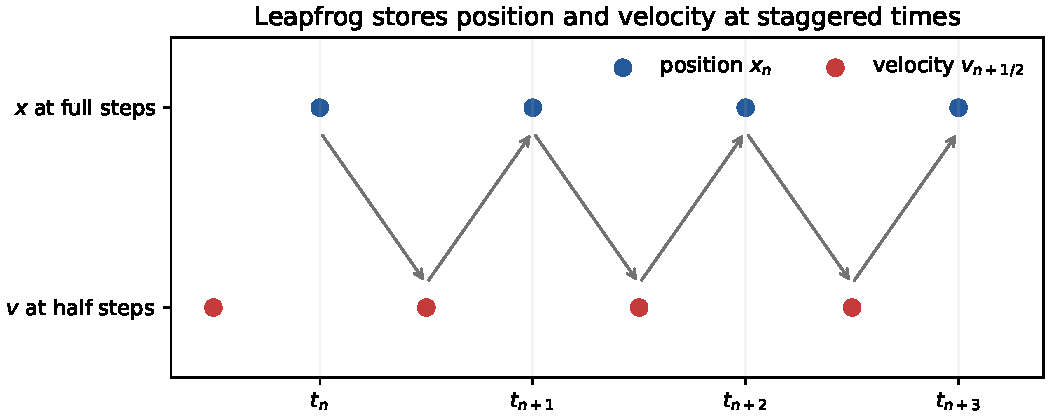
\includegraphics[width=0.78\linewidth]{leapfrog_timing.pdf}
  \end{center}
\end{frame}

\begin{frame}[t]{速度Verlet法}
  MDではleapfrogと等価な速度Verlet表示をよく使う。
  \[
    \begin{aligned}
      \mathbf r_{n+1}&=\mathbf r_n+h\mathbf v_n+\tfrac12h^2\mathbf a_n,\\
      \mathbf v_{n+1}&=\mathbf v_n+\tfrac12h(\mathbf a_n+\mathbf a_{n+1}),\\
      \mathbf a_{n+1}&=\mathbf F(\mathbf r_{n+1})/m.
    \end{aligned}
  \]
  \begin{itemize}
    \setlength{\itemsep}{1mm}
    \item 保存する位置と速度が同じ時刻にそろう
    \item 滑らかな保存力に対して時間反転対称・シンプレクティック
    \item エネルギーは厳密には一定でなく、有限刻みによる誤差を持つ
  \end{itemize}
\end{frame}

\begin{frame}[t]{初期状態：格子配置とMaxwell分布}
  \begin{columns}[T,onlytextwidth]
    \column{0.48\textwidth}
    \begin{itemize}
      \setlength{\itemsep}{1.5mm}
      \item 粒子の重なりを避けるため格子上に配置
      \item 速度成分は平均0、分散$k_{\rm B}T_0/m$の正規分布
      \item 重心速度は差し引かず、温度の自由度を$3N$とする
    \end{itemize}
    \column{0.49\textwidth}
    \centering
    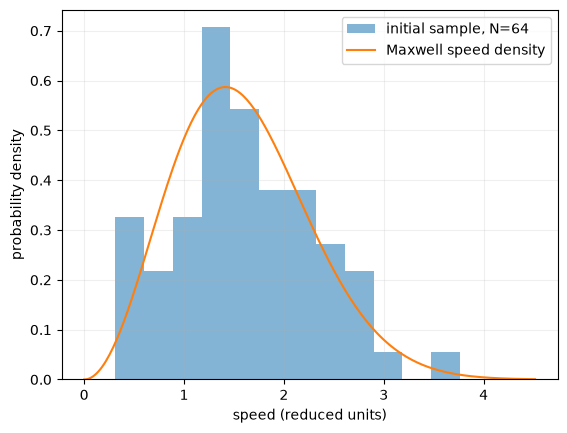
\includegraphics[width=\linewidth]{md_speed_distribution.png}
  \end{columns}
  \small 実線はMaxwellの速さ分布。棒は$N=64$粒子の初期速度標本。
\end{frame}

\begin{frame}[t]{運動エネルギー・温度・圧力}
  \[
    K=\sum_i\frac12m|\mathbf v_i|^2,
    \qquad
    T_{\rm kin}=\frac{2K}{3Nk_{\rm B}}
  \]
  \[
    P=\rho k_{\rm B}T_{\rm kin}
      +\frac{1}{3V}\sum_{i<j}\mathbf r_{ij}\cdot\mathbf F_{ij}
  \]
  \begin{itemize}
    \setlength{\itemsep}{1mm}
    \item 第2項をビリアル圧力寄与と呼ぶ
    \item 圧縮因子$Z=P/(\rho k_{\rm B}T_{\rm kin})$は理想気体で1
    \item $Z$は等温圧縮率$\kappa_T$とは別の量
  \end{itemize}
\end{frame}

\begin{frame}[t]{MDシミュレーションの設定}
  \begin{itemize}
    \setlength{\itemsep}{2mm}
    \item $N=64$、密度$\rho=0.1$、立方体箱
    \item $T_0=1$の正規分布から初期速度を生成（seed固定）
    \item 速度Verlet法、$h=0.01$、1000ステップ
    \item 最小像、$r_c=L/2$のforce-shifted LJ相互作用
  \end{itemize}
  \begin{lessonbox}
    この短いNVE計算は相図の相境界を求める計算ではない。
    粒子数と時間が小さいため、温度・圧力の系列には大きな揺らぎが残る。
  \end{lessonbox}
\end{frame}

\begin{frame}[t]{エネルギーの時間変化}
  \centering
  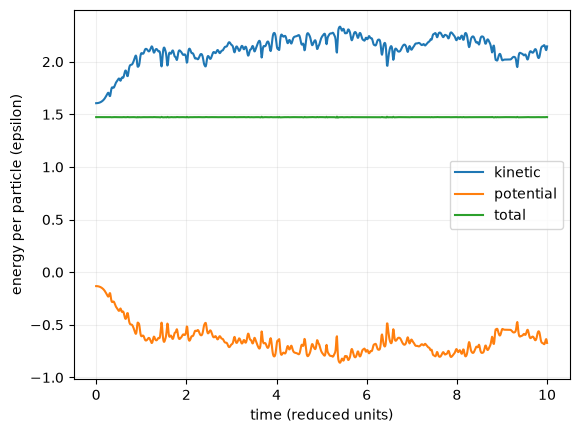
\includegraphics[width=0.67\linewidth]{md_energy.png}

  {\small $N=64$の実行。最大変動は粒子あたり$4.805\times10^{-3}$。\par}
\end{frame}

\begin{frame}[t]{運動学的温度}
  \centering
  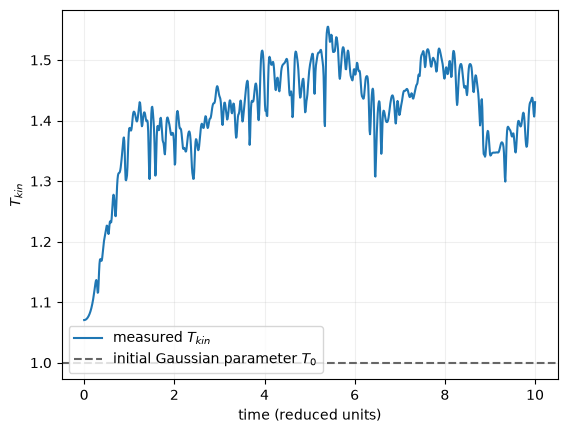
\includegraphics[width=0.67\linewidth]{md_temperature.png}

  {\small 初期の実測温度$1.070$。分布パラメータは$T_0=1$。\par}
\end{frame}

\begin{frame}[t]{圧力と圧縮因子}
  \centering
  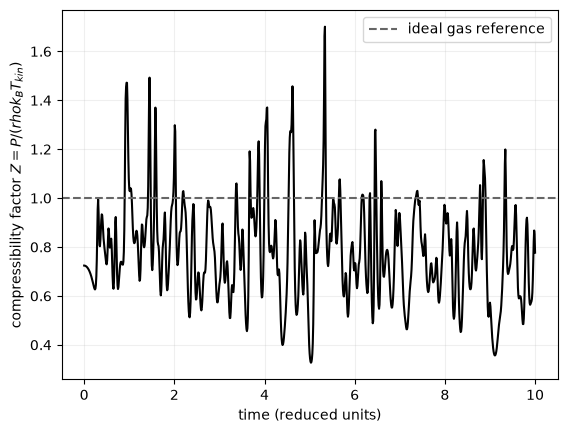
\includegraphics[width=0.67\linewidth]{md_pressure.png}

  {\small $Z=P/(\rho k_{\rm B}T_{\rm kin})$。破線$Z=1$は理想気体の基準。\par}
\end{frame}

\begin{frame}[t]{実習の進め方}
  \begin{enumerate}
    \setlength{\itemsep}{2.5mm}
    \item Lorenz方程式で初期値を変えて軌道間距離を比べる
    \item 二重振り子の初期角を変えて運動とエネルギー誤差を確認する
    \item MDで密度、初期温度、時間刻みを変える
    \item エネルギー、温度、圧力の定義と時間変化を説明する
  \end{enumerate}
  \vspace{2mm}
  \small 分子動力学は粒子数の2乗とステップ数に比例して計算量が増える。
\end{frame}

\end{document}
